\documentclass[10pt,oneside]{book}

\usepackage{MXBookEN}

%% ----------------------------------------
%%   Document Properties
%% ----------------------------------------
\renewcommand{\DocTitle}{Configuration Status Register (CSR) Design Automation}
\renewcommand{\DocDescription}{In-house tool reference manual }
\renewcommand{\DocAuthor}{Xin Meng}
\renewcommand{\DocRevision}{0.0}

%% ----------------------------------------
%%   Document specific defintions
%% ----------------------------------------
\usepackage{shortcut-sv}
\usepackage{shortcut-p2}


%% Glossaries
\makeglossaries
\loadglsentries[main]{gls-xregister.sty}





%% ------------------------------
%%   Document
%% ------------------------------
\begin{document}
\input{MXCover.tex}
%% \input{ExarLegalDisclaimer.tex}
\tablefirsthead{%
  \hline
  \multicolumn{1}{|p{.1\textwidth}}{\tableheader{Revision}}&
  \multicolumn{1}{p{.1\textwidth}}{\tableheader{Date}}&
  \multicolumn{1}{p{.592\textwidth}}{\tableheader{Description}}&
  \multicolumn{1}{p{.1\textwidth}|}{\tableheader{Author}}\\
  \hline}

\tablehead{%
  \hline
  \multicolumn{4}{|l|}{\textsl{...Continued from previous page}}\\
  \hline
  \multicolumn{1}{|p{.1\textwidth}}{\tableheader{Revision}}&
  \multicolumn{1}{p{.1\textwidth}}{\tableheader{Date}}&
  \multicolumn{1}{p{.592\textwidth}}{\tableheader{Description}}&
  \multicolumn{1}{p{.1\textwidth}|}{\tableheader{Author}}\\
  \hline}
\tabletail{%
  \hline
  \multicolumn{4}{|l|}{\textsl{Continued on next page...}}\\
  \hline}
\tablelasttail{\hline}

\begin{supertabular}{|p{.1\textwidth}|p{.1\textwidth}|p{.592\textwidth}|p{.1\textwidth}|}


%% \hyperref[sec:chg log 0.1]{0.1} & 
%% 6/13/2007 & 
%% 2nd draft version for review. & 
%% Xin Meng \\
%% \hline


0.0 & 6/28/2013 & Initial version. & Xin Meng\\

\end{supertabular}


\frontmatter
\tableofcontents
\listoftables
\listoffigures
%% \listofalgorithms
%% \lstlistoflistings

\mainmatter

\chapter{Introduction}\label{sec:chapter intro}
\emph{Control/Status Register} (CSR) is a basic module in chip design. 
It is an interface between software and hardware. Although it is a 
functionally simple module, several design challanges are identified 
during our complex chip development projects:
\begin{enumerate}
\item \textbf{CDC} (clock domain crossing). There are many functional 
  blocks operating in different clock domains. CSR must propagate 
  control/status to/from those clock domains. CDC issues, such as 
  reconvergence or meta-stability can leads to chip functional failure. 

\item \textbf{Address Decoding}. For a complex chip, there will be a 
  large number of registers mapped into software accessible address
  space, which leads to a large decoder and a large MUX. Although CSR
  module is simple, such large logic could also have timing issue. 

\item \textbf{Content Mapping}. In addition to CSRs, other contents 
  such as on-chip memory, register in 3rd party IPs, etc., are expected 
  to be mapped into CSR address space for debugging purpose, which 
  requires a unified protocol for forwarding access to 3rd party IPs.

\item \textbf{Multiple Master}. There could be more than one access masters
  that initiate CSR access. CSR module should architecturally support this. 

\item \textbf{Design/Verification Effort}. CSR is under frequent change
  during chip development. And it is the source for verification, 
  documentation, software development. Maintenance effort should be minimized. 
\end{enumerate}

This document proposes an CSR architecture and an automation methodology to 
address above challanges. This document is organized as follow:
\begin{itemize}
\item \autoref{part:man} provides full description about the usage
  of this methodology, including RTL and testbench architecture, 
  XSD structure, generated files, and command line option. 
\item \autoref{part:imp} documents implementation of methodology, 
include Perl and Python scripts, class hierarchy, etc. 
\end{itemize}



\part{Tool Reference Manual}\label{part:man}
\chapter{CSR Architecture}\label{sec:chapter arch}
\section{Centralization vs. Daisy Chain}
\insertfigure{CSR architecture}{arch}{fig:arch}
As shown in \autoref{fig:arch}, traditionally, Access master maintains
central address decoder and fans out request to each
\gls{target}. Each different \gls{target} has its own CSR access
interface and fans in response to master. If chip has many \gls{target}s
and masters, there could be routing congestion. Such congestion becomes a 
headache especially when we put chip 
on emulation platform, where chip partition is required and connection between
FPGA devices are limited.

In this methodology, \emph{Daisy Chain} architecture is proposed. All \gls{target}s
are chained together to eliminate routing congestion, so each master only has one
pair of fan-in and fan-out. CSR access request is passed through the chain:
\begin{itemize}
\item If a \gls{target} receives a access request targetting CSR belonging to it, access is accepted, 
  \gls{target} produces access completion and passes it to next chain stage. 
\item If a \gls{target} receives a access request targetting CSR not belonging to it, 
  access is bypassed to next chain stage.
\item If a \gls{target} receives a access completion, it bypasses it to next chain stage. 
\item If \gls{master} receives access completion, CSR access transaction is considerted to be 
  finished successfully. It returns result to higher level. 
\item If \gls{master} receives access request, CSR access is failed due bad address
  (no target claims the request), \gls{master} reports error to higher level. 
\item If timeout occurs at \gls{master} during waiting access completion, \gls{master}
  sends flush request to avoid deadlock. (See \autoref{sec:deadlock avoidance})
\end{itemize}
Daisy Chain scheme has following advantages:
\begin{enumerate}
\item Master has constant fan-in and fan-out, routing issue is eliminated, scalability is good.
\item Address decoder and read data MUX are distributed across the chain, 
  potential timing issue is eliminated. 
\item CSR are in implemented their corresponding \gls{target} clock domain, 
  no CDC issues for control signals. 
\item Use standard CDC module to isolate \gls{master} and \gls{target} 
  clock domain, clean for CDC verification.
\item Partition friendly for emulation. 
\end{enumerate}
However, Daisy Chain has a big disadvantage: respond time or CSR access latency
is larger than centralized architecture. Because each access must go through all
chain stages.

\section{Contents to be Mapped}
There are two major types of \emph{contents} in chip that would be accessed
by external entities (such as software, debug facility, etc): registers and 
memories. Contents are packed together and mapped into flatterned 
address spaces for well organized access. Different access permissions are
imposed on contents, such Read-Write, Read-Only, etc. Same contents could be
mapped into several different address spaces with different access permissions. 

For a very complex chip, there are various 3rd party modules that have their
own pre-defined register blocks, these register blocks have their own fixed
packing order and should also be mapped into address space together with other
contents locally developped. For better distinguishing,  these register blocks 
in 3rd party IPs are named ``\emph{\gls{reg file}}'' in this document. ``\emph{Register}''
indicates locally coded ones. 

\section{CSR Access Master}
\gls{csr master} is the initiator that starts register access on 
behalf of higher layer entity. It bridges higher layer entity and
chip registers. 
For example, if chip registers are
mapped into PCIe memory space, host system is a higher layer entity. 
A \gls{csr master} must exist to access registers on behalf of 
host system. It will translate PCIe MRd/MWr to register access and 
return data to host over PCIe link. 
Another example, if chip registers are designed to accessible over
JTAG or UART debugging port. The JTAG/UART port is the higher 
layer entity. A \gls{csr master} must exist to access regiters on behalf 
of JTAG/UART. 

\subsection{Address Space}
One \gls{csr master} can have several separated address spaces. Each
address space can have different mappings, which means same \gls{word}
may have different address in different space. Address space can also
impose additional write protections. For example, Panther2 maps all its 
registers into PCIe BAR0 memory space. So there is a \gls{csr master}
on behalf of host Root Complex. Additionally, PCIe has one PF BAR0 and 
128 VFs BAR0. So this master has 129 address spaces. \gls{word}s are
mapped into all these spaces. And for some \gls{word}s, only PF can 
write, VF can only read. So there are write protection applied on 
VF BAR0 space mappings. 
\subsection{Deadlock Avoidance}\label{sec:deadlock avoidance}
Because there is ``ACK protocol'' between read/write access and 
mapped contents (such as memory), there could be deadlock or hangup 
if internal logic doesn't respond to register access. This will never
happen when access to pure registers because corresponding ACK is 
always asserted. Such assertion is guaranteed by address decoder. 

If unfortunately, deadlock occurs at a specific \gls{csr slave}, 
timeout event is triggered at \gls{csr master}. \gls{csr master}
will then transmit a \emph{flush request} to its daisy chain to 
cancel any halted access and reset all \gls{csr slave} back to normal
state. 

For any \gls{csr slave} that receives flush request, it resets read control
and write control, cancel completion construction and forward flush request 
to next stage. There could racing condition that flush request and 
access completion comes at same cycle, in such condition, completion is 
also discarded. 

Completion construction is triggered by ACK assertion and qualified
by corresponding read/write control signal. This guarantees discard of 
staled ACK. 
For exmaple, 
It is possible internal logic returns access result at later time, and 
corresponding ACK signal will be asserted after flush option is executed. 
Because corresponding read/write control signals has been cleared upon 
flush operation, this ACK will be gated off. 




\section{Field}
\begin{figure}[bthp]
  \centering
  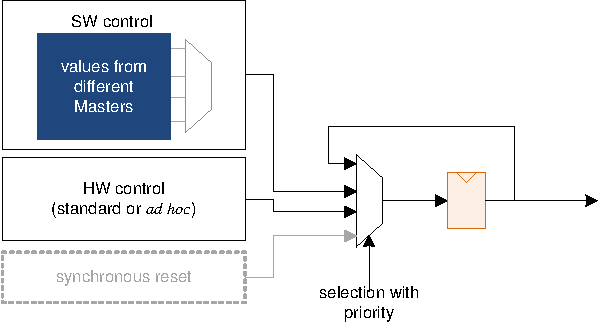
\includegraphics[width=0.6\textwidth]{field}
  \caption{Field RTL block diagram}\label{fig:field}
\end{figure}

\autoref{fig:field} shows general RTL structure of a \gls{field}. 
Field is a Flip Flop (FF) with a bunch of combinational logic in
front of it. If a \gls{field} is mapped into software writable
address space, it can be written by address space \gls{master}s, 
shown in ``SW control'' block.
Hardware can of course update \gls{ff} via design-sepcific logic, 
shown in ``HW control'' block. 
Some field might have synchronous reset requirement, shown 
in dashed line block. 
Each block provides a ``next value'' of field and a MUX with 
pre-defined priority chooses the winner to update field's value.

\subsection{Software Access Type}
From software's perspective, access to a \gls{field} can be well 
abstracted as follow: 
\gls{register-type-read-write}, 
\gls{register-type-read-only}, 
\gls{register-type-read-clear}, 
\gls{register-type-read-write-1-clear}, 
\gls{register-type-read-write-1-set}, 
\gls{register-type-clear-on-conf}, and 
\gls{register-type-write-on-conf}. Follow link on them to get 
the detailed descriptions. 


\subsection{Hardware Access Type}
Hardware access type is more complicated than software access. It
is hard to abstract clearly as that for software because hardware
could have various design specific requirement when accessing field. 
For example, there could be cross reference between different fields, 
filed\_A value change depends on field\_B. 
However, it is possible to abstract some basic hardware control 
scenarios that are commonly used everywhere: 
\begin{enumerate}
\item \gls{hw-register-type-ps}/\gls{hw-register-type-pc}, in which \gls{field} is set or cleared 
  when control signal asserts for a single clock cycle. 
\item \gls{hw-register-type-pv}, in which \gls{field} is set to a specific
  value when control signal asserts for a single clock cycle. 
\item \gls{hw-register-type-pi}/\gls{hw-register-type-pd}, in which \gls{field} is incremented or 
decremented its value when control signal asserts for a signal clock cycle. 
\item \gls{hw-register-type-rtv}, in which \gls{field} is dynamically refreshed
  by a hardware internal signal during operation.
\end{enumerate}

\section{Mapping}
\insertfigure{Field concatenation and mapping}{map}{fig:map}
As shwon in \autoref{fig:map}, individual \gls{field}s are concatenated
together to form a fixed length \gls{word}. \gls{word}s are grouped together
and assigned addresses for \gls{master} access.  
There could be multiple address spaces for different \gls{master}s. So same 
\gls{word} can have multiple addresses. Even a same \gls{field} can be concatenated
several times in different \gls{word}. Accesses from different \gls{master}s are 
decoded and multiplexed. 

So the net effect of concatenation and mapping is to transfer read/write access
from \gls{csr master} down to \gls{field}. One \gls{field} has one or more 
wrapping \gls{word}, each \gls{word} is further mapped into one or more address
spaces, and each space delivers read/write access from \gls{csr master}.

\section{Alignment}
Intuitively, address spaces are byte array. But contents (\gls{word},
memory, or \gls{reg file}), are all multi-byte packed blocks, so
alignment is very important.  For compatible with existing software
model, contents are at least 4-Byte aligned.  For memories and
\gls{reg file}s, in order to save decoding logic, starting address of
them are aligned at their total length. e.g., when a 512bit memory is
mapped, its starting address is aligned at 64B boundary, such as
\mhdl{0x0040} or \mhdl{0x0080}.  Thus lower 6-bit address can be
directly used as memory access address.  Such alignment rule is
mandatory in this architecture.

\section{CSR Access Slave}
\insertfigure{CSR Access Slave in target domain}{access-slave}{fig:access-slave}
As shown in \autoref{fig:access-slave}, \gls{csr slave} decodes \gls{csr master}
access, and executes 4-byte aligned \gls{word} read/write.
For locally developped registers, such access can be guaranteed successfully 
completed unconditionally, otherwise, there is bug in RTL implementation. 

\emph{Decoder} decodes address bus value
to one-hot selection signals for read/write control generation. Depending on 
mapped contents, read/write access have acknowledge. 

If a \gls{target} has hundreds (maybe thousands) of \gls{word}, read MUX could be
critical timing path. In such situation, read MUX must be split into two levels 
to improve timing, as shown in \autoref{fig:mux-split}. Blue MUX and its selection
bus is split into three sub-groups, one extra level (colored as orange) is added. 
\insertfigure{Scalable MUX split}{mux-split}{fig:mux-split}

\SetAlFnt{\small}
\SetAlCapFnt{\small}
\SetAlCapNameFnt{\small}
\begin{figure}[hbtp]
  \begin{algorithm}[H]
    \If{have access request}{
      \If{in address range}{
        \If{access is write}{
          \If{word is protected in the space}{
            Return Bad Write completion\;
          }
          \Else{
            Execute write access\;
          }
        }
        \Else(\emph{access is read}){
          \If{word is protected in the space}{
            Execute normal read\;
          }
          \Else{
            Execute normal read\;
            Assert rd\_req for potential read side effect\;
          }
        }
      }
      \Else(\emph{Not in address range}){
        Forward request to next stage in chain\;
      }
    }
    \ElseIf{have flush request}{
      \If{Completion is being sent}{
        Racing between flush and completion, completion wins\;
      }
      \Else{
        Clear request, forward flush request\;
      }
    }
    \caption{Access execution flow}\label{alg:access}
  \end{algorithm}
\end{figure}

\insertfigure{Read access over slave}{slave-rd}{fig:slave-rd}
\insertfigure{Write access over slave}{slave-wr}{fig:slave-wr}



\section{CSR Access Bridge}
\insertfigure{CSR Access Bridge in target domain}{access-bridge}{fig:access-bridge}
Different from locally developped registers, access \gls{reg file}s or memories
through daisy chain is more complicated. Because \gls{reg file} and memory have
their own access port, and this port could be shared with other existing masters, 
so access from daisy chain may not be completed immediately due to arbitration. 
\gls{csr bridge}, as shown in \autoref{fig:access-bridge},
is thus introduced to bridge daisy chain \gls{csr master}s to \gls{reg file} 
and memories. 

\insertfigure{Read access over bridge}{bridge-rd}{fig:bridge-rd}
\insertfigure{Write access over bridge with flush}{bridge-wr-flush}{fig:bridge-wr-flush}


\section{Value Deliver}
\gls{value deliver} is a toggle based FIFO interface compliant
CDC standard module that provides for delivering value from one
clock domain to another. All flags are active high. 
It's RTL structure is illustrated in \autoref{fig:value-deliver}.

\insertfigure{Toggle based FIFO interface compliant value deliver}
{value-deliver}{fig:value-deliver}

\begin{figure}[bthp]
  {\small
    \begin{tabular}{cc}
      \includegraphics[width=.45\textwidth]{value-deliver-push} &
      \includegraphics[width=.45\textwidth]{value-deliver-pop} \\
      (push FSM) & (pop FSM)\\
    \end{tabular}
  }
  \caption{Value Deliver push/pop FSM}\label{fig:value-deliver-fsm}
\end{figure}

\subsection{Push}
At push side (shaded as orange), there are three ports \mhdl{rdy}, 
\mhdl{vld} and \mhdl{din} that behave as a standard FIFO: when 
\mhdl{rdy} is asserted, it is ready accept next value. User logic
drives next value on \mhdl{din} and asserts \mhdl{vld} for one cycle, 
next value is flopped in and start CDC transfer. \mhdl{req} signal
toggles to indicate next value is ready at push side. 


\subsection{Pop}
At Pop side (shaded as green), once it detects toggle on \mhdl{req},
it flops in value from push domain and asserts \mhdl{vld} to user 
logic. In the meanwhile, it toggles \mhdl{ack} to signal push side
that value has been successfully transferred, and push side can be 
ready for next value. 
During waiting for user logic to fetch value at \mhdl{dout}, push
side could have a new value transferred. In this scenario, pop
side has an internal flag to save the extra ``req''. When current
value is popped by user logic, pop side flops in the new value 
immediately and toggles \mhdl{ack} again. And \mhdl{vld} is kept
asserted to indicate user logic there is yet another value available.




\section{Parameterized MUX}
Core logic in CSR is multiplexier, with/without selection priority. 
Script can generate MUX in Verilog code with \mhdl{case} statement. 
But such scheme pushes all logic into scripts, each generated MUX
needs to be verified, which is not automation. The benefit of 
parameterized modules is they just only need to be verified once, 
then any parameterized instatiation is guaranteed to be correct. 

Essentailly, MUX is a two-level \mhdl{AND} and \mhdl{OR} logic, as 
shown in \autoref{fig:mux}. Each \mhdl{din} vector is \mhdl{AND}'ed
with its selection signal, then all \mhdl{din} vectors are \mhdl{OR}'ed
together to get the \mhdl{dout}. 
\insertfigure{Logic view of MUX}{mux}{fig:mux}

%% \begin{figure}[btph]
%%   \centering
%%   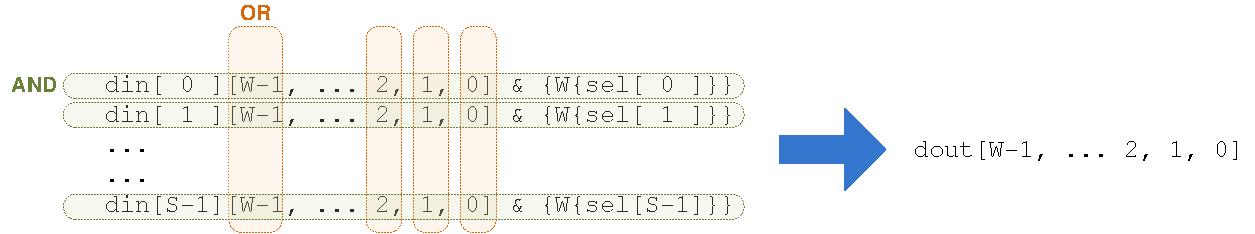
\includegraphics[width=.65\textwidth]{mux}
%%   \caption{Logic view of MUX}\label{fig:mux}
%% \end{figure}

Consider \mhdl{din} as a 2-demension array, \mhdl{AND} calculations
are applied on rows, \mhdl{OR} calculations are applied on columns. 
Verilog unary logic operators \mhdl{&} and \mhdl{|} can only be
applied on vector, they can't take bits across vectors. So the trick
is to transform the matrix with \mhdl{generate} statement for using
unary operators. \autoref{code:one-hot-mux} and 
\autoref{code:priority-mux} are two parameterized MUX implemetations
used in CSR code generation. The One-Hot MUX has been used in DMA
CoS design of Panther2

\lstinputlisting[
  caption={One-Hot parameterized MUX}, 
  label={code:one-hot-mux}, 
  language=metahdl, 
  texcl]{/home/xinmeng/mxmf/projects/xregister/src/one_hot_mux.v}

\lstinputlisting[
  caption={Priority parameterized MUX}, 
  label={code:priority-mux}, 
  language=metahdl, 
  texcl]{/home/xinmeng/mxmf/projects/xregister/src/priority_mux.v}


\section{Packet Format}
\gls{csr master} accesses \gls{csr slave} via packets, \autoref{ds:packet}
illustrates all five packet formats used by them. Packet format is defined 
at 2B (16-bit) boundary. Fields in packet definition are described as follow:
\begin{enumerate}
\item Completion (C), \mhdl{1'b1} means packet is a access
  completion, \mhdl{1'b0} means packet is a request. 

\item Write (W), \mhdl{1'b1} means packet is a write access, 
  \mhdl{1'b0} means packet is a read access. 

\item Completion Status Code (CSC). For 
  a completion, this field further describes the packet contents, 
  valid encoding are:\\
  {\small
    \begin{tabular}{rp{0.7\textwidth}}
      \mhdl{4'b0000} & Successful read completion, there is read data
      contained in packet as illustrated in \autoref{ds:packet}(b). \\

      \mhdl{4'b0001} & Successful write completion, there is no data 
      contained as illustrated in \autoref{ds:packet}(d).\\

      \mhdl{4'b0010} & Bad write completion due to write to protected \gls{word}s.
      There is read data contained
      in packet as illustrated in  \autoref{ds:packet}(d). \\

      \mhdl{4'b0011} & Bad write completion, due to violate \gls{reg file} or 
      memory access protocol. There is no data 
      contained as illustrated in \autoref{ds:packet}(d).\\

      \mhdl{4'b0100} -- \mhdl{4'b1111} & Reserved \\
    \end{tabular}
  }

\item byte\_addr[15:0] is the byte address of target regsiter to be accessed. 
  Because registers are only allowed to be accessed at 4B boundary, so 
  byte\_addr[1:0] are reserved. 

\item rd\_data[31:0] is the read data of read access.
\item wr\_data[31:0] is the write data of write access. 
\end{enumerate}

\begin{figure}[hbtp]
  {\scriptsize
    \begin{bytefield}[bitwidth=0.028125\textwidth, bitheight=.5cm]{16}
      %% \bitbox[lr]{1}{31}\bitbox[lr]{1}{30}\bitbox[lr]{1}{29}\bitbox[lr]{1}{28}\bitbox[lr]{1}{27}\bitbox[lr]{1}{26}\bitbox[lr]{1}{25}\bitbox[lr]{1}{24}
%% \bitbox[lr]{1}{23}\bitbox[lr]{1}{22}\bitbox[lr]{1}{21}\bitbox[lr]{1}{20}\bitbox[lr]{1}{19}\bitbox[lr]{1}{18}\bitbox[lr]{1}{17}\bitbox[lr]{1}{16}
\bitbox[lr]{1}{15}\bitbox[lr]{1}{14}\bitbox[lr]{1}{13}\bitbox[lr]{1}{12}\bitbox[lr]{1}{11}\bitbox[lr]{1}{10}\bitbox[lr]{1}{9}\bitbox[lr]{1}{8}
\bitbox[lr]{1}{7}\bitbox[lr]{1}{6}\bitbox[lr]{1}{5}\bitbox[lr]{1}{4}\bitbox[lr]{1}{3}\bitbox[lr]{1}{2}\bitbox[lr]{1}{1}\bitbox[lr]{1}{0}\\

      \bitbox{12}{\tiny space\_id[11:0]}
      \colorbitbox{gray}{2}{}
      \bitbox{1}{\tiny C=\textcolor{red}{0}}
      \bitbox{1}{\tiny W=\textcolor{red}{0}}\\
      \wordbox{1}{\tiny byte\_addr[15:0]}\\
      \wordbox[]{1}{(a) read request}\\
    \end{bytefield}
    \hfill
    \begin{bytefield}[bitwidth=0.028125\textwidth, bitheight=.5cm]{16}
      %% \bitbox[lr]{1}{31}\bitbox[lr]{1}{30}\bitbox[lr]{1}{29}\bitbox[lr]{1}{28}\bitbox[lr]{1}{27}\bitbox[lr]{1}{26}\bitbox[lr]{1}{25}\bitbox[lr]{1}{24}
%% \bitbox[lr]{1}{23}\bitbox[lr]{1}{22}\bitbox[lr]{1}{21}\bitbox[lr]{1}{20}\bitbox[lr]{1}{19}\bitbox[lr]{1}{18}\bitbox[lr]{1}{17}\bitbox[lr]{1}{16}
\bitbox[lr]{1}{15}\bitbox[lr]{1}{14}\bitbox[lr]{1}{13}\bitbox[lr]{1}{12}\bitbox[lr]{1}{11}\bitbox[lr]{1}{10}\bitbox[lr]{1}{9}\bitbox[lr]{1}{8}
\bitbox[lr]{1}{7}\bitbox[lr]{1}{6}\bitbox[lr]{1}{5}\bitbox[lr]{1}{4}\bitbox[lr]{1}{3}\bitbox[lr]{1}{2}\bitbox[lr]{1}{1}\bitbox[lr]{1}{0}\\

      \colorbitbox{gray}{8}{}
      \bitbox{4}{\tiny CSC}
      \colorbitbox{gray}{2}{}
      \bitbox{1}{\tiny C=\textcolor{red}{1}}
      \bitbox{1}{\tiny W=\textcolor{red}{0}}\\
      \wordbox{1}{\tiny rd\_data[15:0]}\\
      \wordbox{1}{\tiny rd\_data[31:16]}\\
      \wordbox[]{1}{(b) read completion}\\
    \end{bytefield}
    \\
    \begin{bytefield}[bitwidth=0.028125\textwidth, bitheight=.5cm]{16}
      %% \bitbox[lr]{1}{31}\bitbox[lr]{1}{30}\bitbox[lr]{1}{29}\bitbox[lr]{1}{28}\bitbox[lr]{1}{27}\bitbox[lr]{1}{26}\bitbox[lr]{1}{25}\bitbox[lr]{1}{24}
%% \bitbox[lr]{1}{23}\bitbox[lr]{1}{22}\bitbox[lr]{1}{21}\bitbox[lr]{1}{20}\bitbox[lr]{1}{19}\bitbox[lr]{1}{18}\bitbox[lr]{1}{17}\bitbox[lr]{1}{16}
\bitbox[lr]{1}{15}\bitbox[lr]{1}{14}\bitbox[lr]{1}{13}\bitbox[lr]{1}{12}\bitbox[lr]{1}{11}\bitbox[lr]{1}{10}\bitbox[lr]{1}{9}\bitbox[lr]{1}{8}
\bitbox[lr]{1}{7}\bitbox[lr]{1}{6}\bitbox[lr]{1}{5}\bitbox[lr]{1}{4}\bitbox[lr]{1}{3}\bitbox[lr]{1}{2}\bitbox[lr]{1}{1}\bitbox[lr]{1}{0}\\

      \bitbox{12}{\tiny space\_id[11:0]}
      \colorbitbox{gray}{2}{}
      \bitbox{1}{\tiny C=\textcolor{red}{0}}
      \bitbox{1}{\tiny W=\textcolor{red}{1}}\\
      \wordbox{1}{\tiny byte\_addr[15:0]}\\
      \wordbox{1}{\tiny wr\_data[31:16]}\\
      \wordbox{1}{\tiny wr\_data[15:0]}\\
      \wordbox[]{1}{(c) write request}\\
    \end{bytefield}
    \hfill
    \begin{bytefield}[bitwidth=0.028125\textwidth, bitheight=.5cm]{16}
      %% \bitbox[lr]{1}{31}\bitbox[lr]{1}{30}\bitbox[lr]{1}{29}\bitbox[lr]{1}{28}\bitbox[lr]{1}{27}\bitbox[lr]{1}{26}\bitbox[lr]{1}{25}\bitbox[lr]{1}{24}
%% \bitbox[lr]{1}{23}\bitbox[lr]{1}{22}\bitbox[lr]{1}{21}\bitbox[lr]{1}{20}\bitbox[lr]{1}{19}\bitbox[lr]{1}{18}\bitbox[lr]{1}{17}\bitbox[lr]{1}{16}
\bitbox[lr]{1}{15}\bitbox[lr]{1}{14}\bitbox[lr]{1}{13}\bitbox[lr]{1}{12}\bitbox[lr]{1}{11}\bitbox[lr]{1}{10}\bitbox[lr]{1}{9}\bitbox[lr]{1}{8}
\bitbox[lr]{1}{7}\bitbox[lr]{1}{6}\bitbox[lr]{1}{5}\bitbox[lr]{1}{4}\bitbox[lr]{1}{3}\bitbox[lr]{1}{2}\bitbox[lr]{1}{1}\bitbox[lr]{1}{0}\\

      \colorbitbox{gray}{8}{}
      \bitbox{4}{\tiny CSC}
      \colorbitbox{gray}{2}{}
      \bitbox{1}{\tiny C=\textcolor{red}{1}}
      \bitbox{1}{\tiny W=\textcolor{red}{0}}\\
      \wordbox[]{1}{(d) write completion}\\
    \end{bytefield}
    \\
    \begin{bytefield}[bitwidth=0.028125\textwidth, bitheight=.5cm]{16}
      %% \bitbox[lr]{1}{31}\bitbox[lr]{1}{30}\bitbox[lr]{1}{29}\bitbox[lr]{1}{28}\bitbox[lr]{1}{27}\bitbox[lr]{1}{26}\bitbox[lr]{1}{25}\bitbox[lr]{1}{24}
%% \bitbox[lr]{1}{23}\bitbox[lr]{1}{22}\bitbox[lr]{1}{21}\bitbox[lr]{1}{20}\bitbox[lr]{1}{19}\bitbox[lr]{1}{18}\bitbox[lr]{1}{17}\bitbox[lr]{1}{16}
\bitbox[lr]{1}{15}\bitbox[lr]{1}{14}\bitbox[lr]{1}{13}\bitbox[lr]{1}{12}\bitbox[lr]{1}{11}\bitbox[lr]{1}{10}\bitbox[lr]{1}{9}\bitbox[lr]{1}{8}
\bitbox[lr]{1}{7}\bitbox[lr]{1}{6}\bitbox[lr]{1}{5}\bitbox[lr]{1}{4}\bitbox[lr]{1}{3}\bitbox[lr]{1}{2}\bitbox[lr]{1}{1}\bitbox[lr]{1}{0}\\

      \colorbitbox{gray}{14}{}
      \bitbox{1}{\tiny C=\textcolor{red}{1}}
      \bitbox{1}{\tiny W=\textcolor{red}{1}}\\
      \wordbox[]{1}{(e) flush request}\\
    \end{bytefield}
  }
  \caption{Register access packet formats}\label{ds:packet}
\end{figure}


\chapter{W3C XML Schema (XSD)}
XML schema (Note ``s'' is \emph{not} capitalized) is 
a description of a type of XML document, typically expressed in terms
of constraints on the structure and content of documents of that type,
above and beyond the basic syntactical constraints imposed by XML
itself. These constraints are generally expressed using some
combination of grammatical rules governing the order of elements,
Boolean predicates that the content must satisfy, data types governing
the content of elements and attributes, and more specialized rules
such as uniqueness and referential integrity constraints.

W3C XML Schema (Note ``S'' is capitalized), published as a W3C
recommendation in May 2001, is one of several XML schema
languages. It was the first separate schema language for XML to
achieve recommendation status by the W3C. Because of confusion between
XML Schema as a specific W3C specification, and the use of the same
term to describe schema languages in general, some parts of the user
community referred to this language as WXS, an initialism for W3C XML
Schema, while others referred to it as XSD, an initialism for XML
Schema Definition. In Version 1.1 the W3C has chosen to adopt
XSD as the preferred name, and that is the name used in this article.

XSD validator is a tool that takes XSD as input and generates a static 
syntax checker. Any XML document can be checked against XSD to guarantee
all rules specified in XSD are met. 

\section{XSD as Data Structure}
CSR is a highly structured hierarchical module. Although its concrete
RTL structure varies depending on number of \gls{word}, \gls{csr master}s, 
\gls{csr slave}s, etc. Its abstract structure can be described in XSD. 
\autoref{fig:xsd-top} is the XSD used to describe CSR. Note each ``+'' 
means the node can be further expanded. 
\insertfigure{XSD top structure}{xsd-top}{fig:xsd-top}

This XSD is designed to support distributed description, that is the entire
CSR architecture can be described in serval XML files, each file contain one 
or more parts of the architecture. It is useful for a large project such as
Panther2, in which each submodule has its own CSR block. 

Each XML file must start with root element ``xregister''.  Under that, zero 
or more \gls{csr master} definitions or \gls{target} definitions can be 
included. So chip architect can create an XML file containing all \gls{csr master}. 
And each submodule owner can create their own XML files for each \gls{target}. 

\subsection{Master}
As shown in \autoref{fig:xsd-master}, \gls{csr master} only needs three variables
to describe:
\begin{enumerate} 
\item \themecolortext{name} is the master module name
\item \themecolortext{space} subtree describes address spaces owned by the master. 
\item \themecolortext{id-value} is the unsigned value of address space. 
  If counter is larger then 1, which means there are multiple similar address space with 
  same size (such as 128 PCIe VF spaces), \themecolortext{id-value} is starting space ID, 
  succeeding address space IDs derived by incrementing.  
\end{enumerate}
\insertfigure{XSD master subtree}{xsd-master}{fig:xsd-master}


\subsection{Target}
\themecolortext{target} subtree (\autoref{fig:xsd-target}) 
contains all elements for describing target domain module. 
\insertfigure{XSD target structure}{xsd-target}{fig:xsd-target}
\begin{enumerate}
\item \themecolortext{name} is the wrapper module name for encapsulating all target 
  domain blocks. 
\item \themecolortext{field} is the subtree for defining a \gls{field}.
\item \themecolortext{word}  is the subtree for defining a \gls{word}.
\item \themecolortext{memory} is the subtree for defining a memory block mapped in 
  register space. 
\item \themecolortext{slave} is the subtree for defining \gls{csr slave}. 
\end{enumerate}
Logically target subtree is a self contained entity. It is allowed to span
a target domain description across several XML files. target subtree with 
with same \textbf{name} will be merged together at processing stage. 

\subsection{Field}
\autoref{fig:xsd-field} shows the structure of field subtree. A target 
subtree can contain unlimited number of field subtree, which means a \gls{target}
can have any number of registers. Variables of each field (or register) 
can be categorized into four parts:
\begin{enumerate}
\item Field identification, including name, description, short-name, field-width. 
\item Field reset behavior, including reset-value, zero or more synchronous-reset.
\item Field access type, including software-access-type, sw-type-alter-signal,
   hardware-access-type, and value-update-priority.
\item Auxiliary key-value pairs for any other purpose, all included in design-hint.  
\end{enumerate}
Detailed descriptions of each control variables are listed below.
\insertfigure{XSD Field structure}{xsd-field}{fig:xsd-field}

\paragraph{name, short-name, field-width and description}
\themecolortext{name} is the human readable name of a field. 
It might contain space and other symbols.
\themecolortext{short-name} is the name used as part of identifier in
source code. If it is not specified, tool will generate it according to a
internal naming convention (See \autoref{sec:naming}). 
\themecolortext{field-width} is a positive number indicating the width 
of the field. 
\themecolortext{description} is a block of text that fully documents the field's functionality and usage, 
which will be included in the generated document. 

\paragraph{reset-value and synchronous-reset} 
\themecolortext{reset-value} is a string that comform to 
Verilog unsigned number syntax, such as \mhdl{3'b000} or \mhdl{4'hF}. 
\themecolortext{synchronous-reset} contains two sub-elements:
\themecolortext{signal} is the synchronous reset signal name, 
and an optional synchronous reset value. Because in somecases, synchronous
reset can have different reset value from asynchronous reset. A \gls{field}
can have any number of \themecolortext{synchronous-reset} subtree. 

\paragraph{software-access-type and sw-type-alter-signal}
\themecolortext{software-access-type} contains a string indicating 
one of software access types (\gls{register-type-read-write}, 
\gls{register-type-read-only}, 
\gls{register-type-read-clear}, 
\gls{register-type-read-write-1-clear}, 
\gls{register-type-read-write-1-set}, 
\gls{register-type-clear-on-conf}, and 
\gls{register-type-write-on-conf}) of the field. 
\themecolortext{sw-type-alter-signal} specifies the control signal 
name for \gls{register-type-clear-on-conf}, and \gls{register-type-write-on-conf}). 





\paragraph{hardware-access-type and value-update-priority}
\themecolortext{hardware-access-type} contains string value
specifies one of hardware access types (
\gls{hw-register-type-ps}, \gls{hw-register-type-pc}, 
\gls{hw-register-type-pi}, \gls{hw-register-type-pd}, 
\gls{hw-register-type-pv}, and \gls{hw-register-type-rtv}). 
If a \gls{field} can be modified by both software and hardware, 
\themecolortext{value-update-priority} controls who wins 
under a racing condition. By default, software dominates the value update. 


\paragraph{design-hint}
This subtree contains auxiliary key-value pairs for design, verification, 
or even software purpose. This subtree doesn't affect \gls{field} functionality. 
Here is the control variable list:
\begin{enumerate}
\item \themecolortext{must-initialize} is a boolean value. If TRUE, 
  the field must be initialized before simulation. 
\end{enumerate}

\subsection{Word}
\autoref{fig:xsd-word} shows the structure of word subtree. 
It specifies field concatenations. In current design, word width 
is fixed at 32-bit. 
\insertfigure{XSD Word structure}{xsd-word}{fig:xsd-word}
\paragraph{name, deprecated} 
\themecolortext{name} is the 
source code name will be used in identifier. In some cases, 
we might want to remove a \gls{word} from design while still keep 
its concatenation for future reference. 
Such word is deprecated and is indicated by boolean variable
\themecolortext{deprecated}. 




\paragraph{concatenation}
\themecolortext{location-lsb} and \themecolortext{location-msb}
specify the location of a segment inside the \gls{word}.
\themecolortext{field-segment-lsb}
and \themecolortext{field-segment-msb} specify the segment of field
to be used in concatenation, because sometimes 32-bit word is just not big enough
to accomodate a large \gls*{field}. 
\paragraph{count}
A positive number under \themecolortext{count} indicates 
the number of physical copies of the word. All fields referened 
by the word are physically duplicated. 


\subsection{Memory}
\autoref{fig:xsd-memory} shows the structure of memory subtree. 
Memory mapped into register spaces are always accessed in 32-bit words, 
regardless of the actual aspect ratio of the internal memory module. 
\insertfigure{XSD Memory structure}{xsd-memory}{fig:xsd-memory}

\subsection{Slave}
\autoref{fig:xsd-slave} shwos the structure of slave subtree. It describes 
a \gls{csr slave} module. The main structure under slave is map subtree. 
It specifies \gls{word} mapping inside a \gls{csr master} accessible 
spaces.  
\insertfigure{XSD Slave structure}{xsd-slave}{fig:xsd-slave}

\paragraph{master-reference}
One slave must have a corresponding master, \themecolortext{synchronous}
element specifies the clock domain relationship between them. 
CDC or normal Value Deliver module is selected based on its value. 

\paragraph{content-reference} 
They are used to reference mapped words or memories into existing memory
spaces. \themecolortext{name} contains a list of referenced contents separated 
by comma to form a group of contents to be mapped.
It is possible words, memories and spaces are defined with \themecolortext{count}
more than one. \themecolortext{id} is used to specify which entities are referenced. 
\themecolortext{id} is a string that specifies number range, such as:
\begin{itemize}
\item 1
\item 1-3
\item 3, 5, 6, 9-12
\end{itemize}
``\mhdl{*}'' is a special pattern that means all instances are referenced. 

\paragraph{space-reference}
Mapping one or more words/memories to one or more spaces, is a kind of traversing of
mapped conetents. Consider following model in \autoref{fig:map}. 
\insertfigure{Content mapping model}{map}{fig:map}

When more than one content names are listed in \themecolortext{content-reference/name} 
element, these names forms a \emph{Content Group} of contents to be mapped, total number 
of contents is denoted as $C$. Each content's \themecolortext{count} could be larger than one, 
which means each content has multiple (say, $N$) instances. The mapping problem is
to linearly put all or some of content $C_{c,n}$, $c \in [0, C-1]$ and $n \in [0,N-1]$, into 
free slots (one slot is a free byte address) of give address space. 
So each content occupies a range of slots  in space $s$, $R_{c,n}^s = [A_{start}, A_{end}]$, 
where $s \in [0,S-1]$, $S$ is the total number of address sapces. 


Intuitively, we traverse content one by one, either \emph{Breadth
  First} or \emph{Depth First} as shown in \autoref{fig:map}. Thus
slots are used one by one. So only starting address $A_0$ needs to be 
specified, all other address can be calculated during traverse. 
But for alignment consideration, contents
should be put at into slots whose address has special alignment
feature. One basic requirement is \gls{word} should be placed at 4B
aligned address. If the content has more than one \gls{word}, such 
as memory, it should be placed at address boundary whose address 
is aligned with its length so as to reduce decode complexity. 
\themecolortext{content-alignment} element is design for this purpose. 
It accepts a list of strings (separated by comma) specifying alignment
requirement for each content in \emph{Content Group}. Default alignment
is 4B. Each sepcifier contains two parts:
\begin{enumerate}
\item Alignment Boundary, that starts with ``A'' and a decimal number or 
  a hex number with leading ``0x''. such as
  \begin{itemize}
    \item A4. Align at 4B boundary
    \item A256. Align at 256B boundary
    \item A0x100. Align at 256B.
  \end{itemize}
  Default value is ``A4''. 

\item An offset, that is a decimal number or hex with leading ``0x''. ``+'' or 
  ``-'' sign must be used to specify positive or negtive offset to the aligned 
  boundary. Then number must be integer multiple of 4. such as
  \begin{itemize}
    \item A256+4. Align at 4B after any 256B boundary, 260B, 516B, etc. 
    \item A0x10-4. Align at 4B before any 16B boundary, 12B, 28B, 44B, etc.  
  \end{itemize}
  Default value is ``+0''.
\end{enumerate}

\SetAlFnt{\tiny}
\SetAlCapFnt{\tiny}
\SetAlCapNameFnt{\tiny}
\begin{figure}[hbtp]
  \begin{minipage}[t]{.31\textwidth}
    \begin{algorithm}[H]
      \ForEach{$s$ in $[0,S-1]$}{
        $A_{base} = A_0^I$\;
        \ForEach{$i$ in $[0,I-1]$}{
          $A_{base} = IAlign(A_{base})$ \;
          $A_{start} = A_{base}+A_0^S$ \;
          \ForEach{$c$ in $[0,C-1]$}{
            \ForEach{$n$ in $[0,N-1]$}{
              $A_{start} = CAlign(A_{start})$\;
              $Allocate(s, A_{start}, size)$ \;
              $A_{start} = A_{start} + size$\;
            }
          }
          $A_{base} = A_{start}$ \;
        }
      }
      \caption{Cartesian:Depth-First traverse}\label{alg:cartesian-d}
    \end{algorithm}
  \end{minipage}
  \hfill
  \begin{minipage}[t]{.31\textwidth}
    \begin{algorithm}[H]
      \ForEach{$s$ in $[0,S-1]$}{
        $A_{base} = A_0^I$\;
        \ForEach{$i$ in $[0,I-1]$}{
          $A_{base} = IAlign(A_{base})$ \;
          $A_{start} = A_{base}+A_0^S$ \;
          \ForEach{$n$ in $[0,N-1]$}{
            \ForEach{$c$ in $[0,C-1]$}{
              $A_{start} = CAlign(A_{start})$\;
              $Allocate(s, A_{start}, size)$ \;
              $A_{start} = A_{start} + size$\;
            }
          }
          $A_{base} = A_{start}$ \;
        }
      }
      \caption{Cartesian:Breadth-First traverse}\label{alg:cartesian-b}
    \end{algorithm}
  \end{minipage}
  \hfill
  \begin{minipage}[t]{.36\textwidth}
    \begin{algorithm}[H]
      \ForEach{$(n,s)$ in $\{(n_0, s_0), (n_1, s_1), \cdots , (n_m, s_m)\}$}{
        $A_{base} = A_0^I$\;
        \ForEach{$i$ in $[0,I-1]$}{
          $A_{base} = IAlign(A_{base})$ \;
          $A_{start} = A_{base} +A_0^S$\;
          \;
          \ForEach{$c$ in $[0,C-1]$}{
            $A_{start} = CAlign(A_{start})$\;
            $Allocate(s, A_{start}, size)$ \;
            $A_{start} = A_{start} + size$\;
          }
          $A_{base} = A_{start}$\;
        }
      }
      \caption{Bijection traverse}\label{alg:bijection}
    \end{algorithm}
  \end{minipage}
\end{figure}

When mapping multiple contents into multiple spaces, two mapping style exist:
\begin{enumerate}
\item \emph{Cartesian}, that maps all contents into all spaces. 
\item \emph{Bijection}, that maps each instance into each spaces, so $N=S$ must
  hold. 
\end{enumerate}
\autoref{alg:cartesian-b} and \autoref{alg:cartesian-d}
shows algorithm for \emph{cartesian} allocating 
slots to contents in 
Breadth-First and Depth-First mode. \autoref{alg:bijection} shows algorithm
for \emph{bijection} allocating slots to contents. 


\paragraph{read-only} 
Add read only protection for the mapped content in the space. 

\paragraph{access-indication}
``RD'', ``WR'', ``ALL'' are three allowed strings, which means 
pulse will be generated when the mapped content is under 
read, write or any access the space. 


\section{Address Mapping}
\pictext{Mapping register across multiple instances}{multi-inst}{fig:multi-inst}{
  \footnotesize
  \put(6,95){$A_{base}^{i1}$}
  \put(3,92.5){$T_1:A_{start}$}
  \put(3,83.5){$T_1:A_{end}$}
  \put(3,76){$T_2:A_{start}$}
  \put(3,68){$T_2:A_{end}$}
  \put(3,64){$T_3:A_{start}$}
  \put(3,62){$T_3:A_{end}$}

  \put(6,59.5){$A_{base}^{i2}$}
  \put(3,57){$T_1:A_{start}$}

  \put(41,84){$A_{base}^{i1}$}
  \put(50,84){$A_{base}^{i1}$}
  \put(59,84){$A_{base}^{i1}$}

  \put(41,58){$A_{base}^{i2}$}
  \put(50,58){$A_{base}^{i2}$}
  \put(59,58){$A_{base}^{i2}$}

  \put(46,36){$A_{base}^{i1}=Ialign(A_0^I)$}
  \put(46,34){$T_1:A_{start}=Calign(A_{base}^{i1}+T_1:A_0^S)$}
  \put(46,32){$T_1:A_{end} = T_1:A_{start}+size -1 $}
  \put(46,30){$T_2:A_{start} = Calign(A_{base}^{i1} + T_2:A_0^S$}
  \put(46,26){$A_{base}^{i2} = Ialign(T_3:A_{end})$}
  
}

\section{XML as Design Synchronization}
\autoref{fig:xml-flow} is the flow chart of XSD/XML based CSR design
automation flow. An XSD aware editor will prompt next element based on
existing element, which turns CSR design to a table filling process.

\insertfigure{XSD/XML based automation flow}{xml-flow}{fig:xml-flow}

All XML files are first validated against XSD, if no error detected, 
a python script will merge and parse all XML files to create a persistent
tree data structure, as shown in \autoref{fig:uml}. 
This tree structure (root is \mhdl{Register} class) is the start point for generating 
other files (code or document), and can be interactively queried for searching
registers, remaining slots in space, etc. 

\insertfigure{UML Class Diagram of python persistent Data Structure}{uml-association}{fig:uml}

\chapter{Naming Convention}\label{sec:naming}
CSR described in XML files only contains core information, there are
a lot of supplementary texts needed for code generation. All rules, a.k.a.
naming convetion, for these texts are built inside various scripts. This chapter
lists all those rules with examples. 

\section{White Space Collapsing}
When typing string in XML, white spaces between words 
are use without limitation, but white spaces are not 
allowed in identifier in source code. So multiple white
spaces are collapsed to single white space, and the single
white space is replaced with underscore `\mhdl{_}'. For 
example, string transformation will be as follow:
\begin{center}
\lstinline[showspaces=true,basicstyle=\tt]{pcie   pf     bar0}
$\rightarrow$ 
 \mhdl{pcie_pf_bar0}
\end{center}

\section{Word Collapsing}
A good human readable name contains several words separated
by white spaces. But a good source code identifier is as short
as possible while still expressive enought for readers to get
the original meaning. Exar RTL SOP defines a dictionary for mapping 
high frequency words to short abbreviations  used in source code, 
such as ``enable'' to ``en'', ``high'' to ``hi'', ``write'' to ``wr'', 
etc. But unfortunately, CSR names are much longer and often
use function spcific words that are not listed in the SOP dictionary.
The XML parser uses following rules (with priority) to 
collapse words to abbreviations:
\begin{enumerate}
  \item For \themecolortext{master/name}, \themecolortext{target/name}, 
    \themecolortext{slave/name}, and \themecolortext{memory/name}, all characters 
    in words are preserved, only white spaces are collapsed. 
    
  \item\label{item:short-name} For \gls{field} and \gls{word}, 
    \begin{enumerate}
      \item if designer specify a \themecolortext{short-name}, parser
        just use it. It is impossible to have short name conflict because 
        XSD declares it as \lstinline{xs:ID} type, validator will check the uniqueness. 
      \item else, parser constructs short name by picking starting characater 
        of each word. If the ultimate abbreviation already exists, a number 
        is suffixed (\mhdl{_2}, \mhdl{_3}, etc.) for distinguishing. 

        For example, \lstinline[showspaces=true]{"command pointer ring  read pointer"}
        is abbreviated as \mhdl{cprrp}. 
    \end{enumerate}

  \item For \gls{word} definition, word short name is created according to 
    rule\autoref{item:short-name}. When word apears in address space context, 
    such as read/write signal generation, word is labeled with its address.
\end{enumerate}



\section{Prefix and Suffix}
To further improve readability when constructing signal from 
parsed names, prefix and suffix are added. Major rules are listed as
below, users can easily interpret other prefix or suffix from generated
code with separation rules (\autoref{sec:separation}). 
\begin{enumerate}
\item \mhdl{mst_} prefix is used for master module name.
\item \mhdl{slv_} prefix is used for slave module name. 
\item \mhdl{tgt_} prefix is used for target module name.
\item \mhdl{s_} prefix is used for address space name. 
\item \mhdl{w_} prefix is used for \gls{word} name.
\item \mhdl{f_} prefix is used for \gls{field} name.
\item \mhdl{m_} prefix is used for memory name. 
\item \mhdl{mem_rd}, \mhdl{mem_rd_data}, \mhdl{mem_wr}, \mhdl{mem_wr_data}, \mhdl{mem_addr}, \mhdl{mem_ack}, 
  suffixes are used for mapped memory access.
\item \mhdl{sel} suffix is used for select signal in decoder.
\item \mhdl{rd} suffix is used for read control signal in read control.
\item \mhdl{wr} suffix is used for write control signal in write control. 
\item \mhdl{wr_data} suffix is used for write data bus in write control.
\item \mhdl{pi}, \mhdl{pd}, \mhdl{pc}, \mhdl{ps}, and \mhdl{rtv} suffixes
  are used for hardware control \gls{hw-register-type-pi}, 
  \gls{hw-register-type-pd}, 
  \gls{hw-register-type-pc}, 
  \gls{hw-register-type-ps}, 
  and \gls{hw-register-type-rtv}, to a \gls{field}, respectively. 
\item \mhdl{pv_ctrl} and \mhdl{pv_value} are suffixes for \gls{hw-register-type-pv}
  control and value signals. 
\item \mhdl{rd_flag} and \mhdl{wr_flag} are suffixes for 
  read and write indication signals. 
\end{enumerate}


\section{Separation}\label{sec:separation}
Underscore ``\mhdl{_}'' is widely used for separating words in source code. 
In \gls{word} name, \gls{field} name, module name, etc, it is heavily used. 
In order to emphsize separation among different parts (names, prefix, suffix) of a 
signal name, we use three consecutive underscores ``\mhdl{___}''. 
Single underscore is used to replace white space
inside a multi words name. Here are some examples of separation and prefix/suffix. 
Note this is NOT the ultimate RTL code generated by script, it is used 
for demonstrating prefix/suffix and separation rules. 
\begin{mhdle}[texcl, caption={Separation and prefix/suffix demo for register content}]
always_ff @(posedge clk or negedge rst_n)
  if (!rst_n)
     f_cpr_wr_ptr[11:0] <= 12'd0;
  else 
     if (w_cpr_wr_ptr___wr) 
        f_cpr_wr_ptr[11:0] <= slv_pcie___wr_data[11:0];
     else 
        f_cpr_wr_ptr[11:0] <= f_cpr_wr_ptr[11:0];

// Three parts in signal name:
//    \textcolor{red}{pcie\_pf\_bar0} is the address space name, \textcolor{red}{s\_} prefix is added,
//    \textcolor{red}{8008} is the mapped address, \textcolor{red}{w\_} prefix is added,
//    \textcolor{red}{sel} is the suffix indicating signal functionality, 
// they are joined with three underscores: \_\_\_
assign s_pcie_pf_bar0___w_8008___sel = slv_pcie___address[15:0] == 16'h8008 && 
                                       slv_pcie___space_id[11:0] == `PF_BAR0;
assign s_pcie_vf0_bar0___w_8008___sel = slv_pcie___address[15:0] == 16'h8008 && 
                                        slv_pcie___space_id[11:0] == `VF0_BAR0;

// \textcolor{purple}{`w\_cpr\_wr\_ptr\_\_\_ack} is a Verilog macro, 
// this coding style is for unification with memory access code.
// For regular register, the macro is defined to \textcolor{red}{1'b1}
always_ff @(posedge clk or negedge rst_n)
   if (!rst_n)
      w_cpr_wr_ptr___wr <= 1'b0;
   else if (w_cpr_wr_ptr___wr && /*- \textcolor{purple}{`w\_cpr\_wr\_ptr\_\_\_ack} -*/ ) 
      w_cpr_wr_ptr___wr <= 1'b0;
   else if (slv_pcie___wr_access && (s_pcie_pf_bar0___w_8008___sel || 
                                     s_pcie_vf0_bar0___w_8008___sel ) )
      w_cpr_wr_ptr___wr <= 1'b1;
   else 
      w_cpr_wr_ptr___wr <= w_cpr_wr_ptr___wr;
\end{mhdle}






\chapter{Target Files Generation}
After XML validation and parsing, python persistent data structure
is generated. Scripts can load the data structure and generate any 
types of file in demand. 

\section{Verilog RTL}
\textsf{gen-rtl.py} is python script for generating Verilog 
RTL source code for \gls{csr master} and \gls{csr slave}, 
which includes \gls{field} and \gls{word}. This section lists
generated codes. 
\subsection{Field without Synchronous Reset}
\lstinputlisting[language=metahdl]{/home/xinmeng/mxmf/projects/xregister/src/field.v}

\subsection{Field with Synchronous Reset}
\lstinputlisting[language=metahdl]{/home/xinmeng/mxmf/projects/xregister/src/field_sync_rst.v}

\subsection{Software Control}
\lstinputlisting[language=metahdl]{/home/xinmeng/mxmf/projects/xregister/src/sw_ctrl.v}

\subsection{Hardware Control}
\lstinputlisting[language=metahdl]{/home/xinmeng/mxmf/projects/xregister/src/hw_ctrl.v}

\subsection{Decoder}
\subsection{Master}
\subsection{Target}


\chapter{Tool Invocation}

\part{Implementation}\label{part:imp}

\appendix
\part{Appendix}\label{part:appendix}
%\chapter{xregister.xsd}
%\lstinputlisting[language=XSLT]{/home/xinmeng/mxmf/projects/xregister/eclipse/register.xsd}

\setglossarysection{chapter}
\printglossary[nonumberlist=true, style=altlist, type=main]



%% \clearpage
%% \refstepcounter{chapter}
%% \addcontentsline{toc}{chapter}{Bibliography}  
%% \label{sec:bib}\bibliography{library}
%% \bibliographystyle{plainurl}

%% \clearpage
%% \refstepcounter{chapter}
%% \addcontentsline{toc}{chapter}{Index}  
%% \label{sec:index}\printindex

\clearpage




\end{document}
